% Copyright (c) 2020 Robert Ryszard Paciorek <rrp@opcode.eu.org>
% 
% MIT License
% 
% Permission is hereby granted, free of charge, to any person obtaining a copy
% of this software and associated documentation files (the "Software"), to deal
% in the Software without restriction, including without limitation the rights
% to use, copy, modify, merge, publish, distribute, sublicense, and/or sell
% copies of the Software, and to permit persons to whom the Software is
% furnished to do so, subject to the following conditions:
% 
% The above copyright notice and this permission notice shall be included in all
% copies or substantial portions of the Software.
% 
% THE SOFTWARE IS PROVIDED "AS IS", WITHOUT WARRANTY OF ANY KIND, EXPRESS OR
% IMPLIED, INCLUDING BUT NOT LIMITED TO THE WARRANTIES OF MERCHANTABILITY,
% FITNESS FOR A PARTICULAR PURPOSE AND NONINFRINGEMENT. IN NO EVENT SHALL THE
% AUTHORS OR COPYRIGHT HOLDERS BE LIABLE FOR ANY CLAIM, DAMAGES OR OTHER
% LIABILITY, WHETHER IN AN ACTION OF CONTRACT, TORT OR OTHERWISE, ARISING FROM,
% OUT OF OR IN CONNECTION WITH THE SOFTWARE OR THE USE OR OTHER DEALINGS IN THE
% SOFTWARE.

\documentclass[a4paper]{article}

\usepackage{tikzPackets}
\usepackage{adjustbox,hyperref,fancyvrb-ex,fvextra}

\oddsidemargin=0pt
\textwidth=430pt

\topmargin=-30pt
\textheight=662pt

\newcommand{\pkgLink}[1]{\texttt{\href{https://ctan.org/pkg/#1}{#1}}}

\fvset{
	breaklines=true,
	breakanywhere=true,
	breakaftersymbolpre={},
	breakaftersymbolpost={\tiny\ensuremath{\ \lhook\joinrel\rightarrow\ }},
	breakanywheresymbolpre={},
	breakanywheresymbolpost={\tiny\ensuremath{\ \lhook\joinrel\rightarrow\ }}
}

\begin{document}

\title{The \texttt{tikzPackets}  package}
\author{Robert Ryszard Paciorek <rrp@opcode.eu.org>}
\date{2020-07-13}
\maketitle

This package provide command for simple build network packets illustration with \pkgLink{tikz}.
Similar functionality (with tables instead of tikz) provide package \pkgLink{bytefield}.

\section{Basic Example}

\begin{CenterExample}
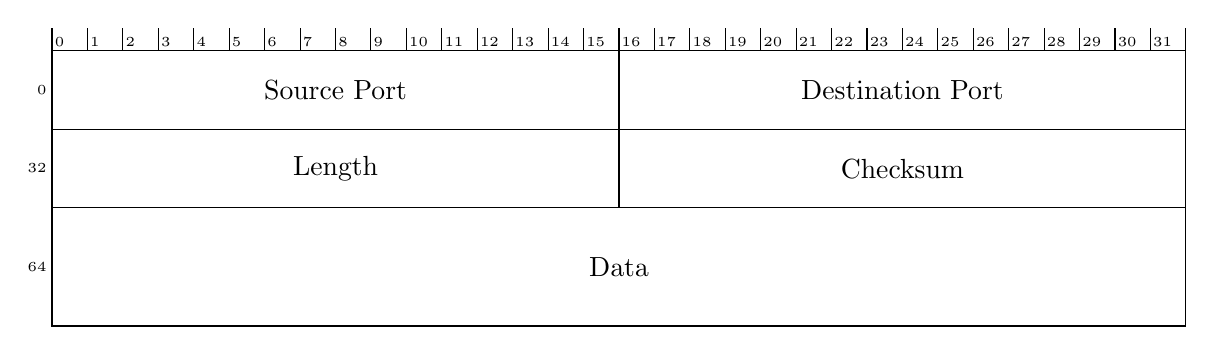
\begin{tikzpicture}
    \packetsInit
    \packetsBitWidth=4.5mm
    \packetsPrintBitScale{31}
    
    \packetsPutField{16}{Source Port}
    \packetsPutField{16}{Destination Port}
    \packetsEndLine{0}{}
    
    \packetsPutField{16}{Length}
    \packetsPutField{16}{Checksum}
    \packetsEndLine{32}{}
    
    \packetsPutField[protocolsField, minimum height=1.5cm]{32}{Data}
    \packetsEndLine{64}{}
\end{tikzpicture}
\end{CenterExample}


\section{Macros description}

\subsection{packetsInit}

\Verb$\packetsInit$ is used to initialise \textit{tikzPackets} variables, counters and tikz styles.
Must be used in every \Verb$tikzpicture$ that use \textit{tikzPackets} package commands before any other \textit{tikzPackets} command.

\subsection{packetsPrintBitScale}

\Verb$\packetsPrintBitScale$ draw bits scale. It takes one argument: last bit value.

Formatting of bits scale can be adjust by redefine (after \Verb$\packetsInit$) tikz style \Verb$bitScaleInfo$, redefine \Verb$\packetsBitFont$ or \Verb$\packetsPrintBitNumber$ macro.

\subsection{packetsPutField}

\Verb$\packetsPutField$ draw packet field. It takes 4 arguments:
\begin{enumerate}
    \item (optional) node style and formatting options
    \item number of bits (width of field)
    \item (optional) node name for new created node
    \item name (text to display)
\end{enumerate}

\subsection{packetsPrintRangeOnLeft and packetsPrintRangeOnRight}

\Verb$\packetsPrintRangeOnLeft$ and \Verb$\packetsPrintRangeOnRight$ prints info (start bit number or bits range) on left or right side of current line.
Should be call after call all \Verb$\packetsPutField$ for this line. Both commands takes two arguments: first bit in line and last bit in line,
but \Verb$\packetsPrintRangeOnLeft$ ignore second argument.

Formatting of printing text can be adjust by redefine \Verb$\packetsBitFont$ macro or redefine \Verb$\packetsPrintRangeOnLeft$ / \Verb$\packetsPrintRangeOnRight$ macros.

\begin{CenterExample}
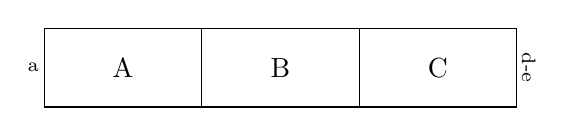
\begin{tikzpicture}
    \packetsInit
    \renewcommand{\packetsBitFont}{\scriptsize}
    \packetsPutField{4}{A} \packetsPutField{4}{B} \packetsPutField{4}{C}
    \packetsPrintRangeOnLeft{a}{b}
    \packetsPrintRangeOnRight{d}{e}
\end{tikzpicture}
\end{CenterExample}

\subsection{packetsNextLine}

\Verb$\packetsNextLine$ end current line of field and prepare to start next line of field. It don't have arguments.

\subsection{packetsEndLine}

\Verb$\packetsEndLine$ call \Verb$\packetsPrintRangeOnLeft$ and \Verb$\packetsNextLine$.
Arguments are passed to \Verb$\packetsPrintRangeOnLeft$.

\subsection{packetsLastNode and packetsFirstNodeInLastLine}

\Verb$\packetsLastNode$ hold name of last added node by \Verb$\packetsPutField$ or \Verb$\packetsPrintBitScale$ (and is used for node positioning in \Verb$\packetsPutField$ and \Verb$\packetsPrintRangeOnRight$ macros).

\Verb$\packetsFirstNodeInLastLine$ hold name of first node (added by macro \Verb$\packetsPutField$ or \Verb$\packetsPrintBitScale$) in current line (and is used in \Verb$\packetsPutField$ and \Verb$\packetsPrintRangeOnLeft$ for positioning)

Both can be use for external to reference node adding by these macros (can be captured after add node by \Verb$\edef$) or can be used to start adding nodes by \Verb$\packetsPutField$ relative to some manually added node.

\begin{CenterExample}
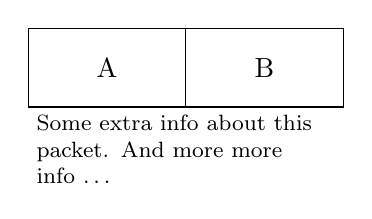
\begin{tikzpicture}
    \packetsInit
    \packetsPutField{4}{A}
    \packetsPutField{4}{B}
    
    \node[
        align=left, anchor=north west,
        text width=7\packetsBitWidth, node font=\footnotesize
    ] [] at (\packetsFirstNodeInLastLine.south west) {
        Some extra info about this packet. And more more info \ldots
    };
\end{tikzpicture}
\end{CenterExample}

\section{Styles and dimmensions}

Width of single bit is set by \Verb$\packetsBitWidth$ and default is 5mm. Default style for node created by \Verb$\packetsPutField$ is \Verb$protocolsField$ and it set line height to 1cm.
Package provide also \Verb$protocolsFieldBase$ style with minimal setting for node style.
Macro \Verb$\packetsBitFont$ define font settings for bits info.
All this change should be done after use \Verb$\packetsInit$.

\begin{CenterExample}
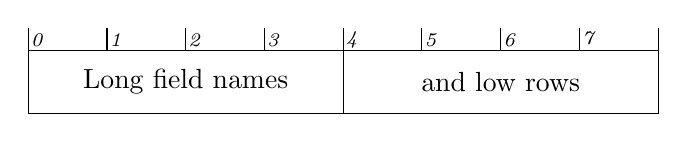
\begin{tikzpicture}
    \packetsInit
    \tikzstyle{protocolsField}=[protocolsFieldBase, draw, minimum height = 0.8cm]
    \packetsBitWidth=10mm
    \renewcommand{\packetsBitFont}{\scriptsize\it}
    
    \packetsPrintBitScale{7}
    \packetsPutField{4}{Long field names}
    \packetsPutField{4}{and low rows}
\end{tikzpicture}
\end{CenterExample}

\end{document}
